\cleardoublepage

% hello
% \includepdf[width=16cm,page=1]{induction-2.pdf}
% \begin{figure}[!h]
\begin{tikzpicture}
    % \fill[black] (0,0) rectangle (5.25in,-7in);

    \node[text width=3in,scale=1.25] at (0,0) {Deep in a cave explorers};% stumbled onto mysterious writing...};
    \node[text width=3in,scale=1.25] at (0,-1) {stumbled onto mysterious writing...};
    \node (A) at (-0.5in,-2in) {
        \includegraphics[width=2.5in]{equiv.png}
    };
    \node at ( 2.5in, -2in) {...on the floor...};
    %
    \node at (0,-5.5in) {
        \includegraphics[width=3in]{total.png}
    };
    \node at ( 0in, -4in) {...on the ceiling...};
    \node at (2in,-4in) {
        \includegraphics[width=2.5in]{ceiling.png}
    };

    \node[text width=2.5in] at ( 2.75in, -5.75in) {...equations, new numbers, and transformations.};

    \node[text width=2.5in,scale=1.25] at ( 1in, -6.75in) {How did it fit together?};
    
\end{tikzpicture}
% \end{figure}

\newpage
~
\vspace{5in}
% \begin{figure}[!h]
\begin{tikzpicture}
    \fill[black] (-2.75in,2.75in) rectangle (2.75in,-2.75in);
    

    %
    \node at (0,0) {
        \includegraphics[width=5in]{context.png}
    };
\end{tikzpicture}
% \end{figure}

\chapter{Noether's Isomorphism Theorems}

\section{A slice of functions}

Sometimes I want to know everything I can about one type 
of data $A$.  Simple type theory tells me that I have functions 
$f:A\to B$ and $g:B\to A$.  So I could begin by exploring 
what these tell me. I am going to focus first on 
functions $f:A\to B$.  


Since I am exploring $A$ and a I have function leaving $A$
it can ask if two terms of $A$ end up in the same place.
\begin{align*}
    a\equiv \acute{a} \pmod{f} & \defeq 
    \bigl(f(a)=_B f(\acute{a})\bigr).
\end{align*}
This is its own function, $\equiv:A\times A\to \mathsf{Prop}$
but now at least it only talks about $A$ (and propositions).
If this construction is familiar then you have been shown 
equivalence relations before.  First we look at the richer syntatic 
qualities.

\begin{theorem}
    Let $a\equiv \dot{a}$ abbreviate $a\equiv \dot{a}\pmod{f}$.
    \begin{description}
        \item[Multiplication] there is a function 
        \[\Box *\Box :\left(a\equiv \acute{a}\right)
        \times \left(\dot{a}\equiv \ddot{a}\right)
        \longrightarrow 
        \left(a\equiv \ddot{a}\right).\]

        \item[Identity] there is an inhabitant of $a\equiv a$ and 
        \begin{align*}
            (a\equiv a)*(a\equiv \dot{a}) &= (a\equiv \dot{a})\\
            (a\equiv \dot{a})*(\dot{a}\equiv \dot{a}) &= (a\equiv \dot{a})
        \end{align*}
        \item[Inverse] there is a function 
        $\Box^{-}:(a\equiv \dot{a})\rightarrow (\dot{a}\equiv a)$ where 
        \begin{align*}
            (a\equiv \dot{a})*(a\equiv \dot{a})^{-} & = (a\equiv a)\\
            (a\equiv \dot{a})^{-}*(a\equiv \dot{a}) & = (\dot{a}\equiv \dot{a})
        \end{align*}
    \end{description}
    In otherwords, $\equiv$ gives the structure of a groupoid.
\end{theorem}
\begin{proof}
    Since $refl_{f(a)}:(f(a)=_B f(a))$, $a\equiv a\pmod{f}=(f(a)=_b f(a))$
    is inhabited.  For $sym$, given $pf:(a\equiv b\pmod{f})$ it follows 
    $pf:(f(a)=_B f(\dot{a}))$.   Hence $pf=refl_{f(a)}:f(a)=_B f(a)$.
    Hence also $pf:f(\dot{a})=_B f(a)$ so that $sym(pf)\defeq pf$ 
    has type $\dot{a}\equiv a\pmod{f}$.
    Finally, for $trans(pf1,pf2)$ observe that 
    $pf1=pf2=refl_{f(a)}$ and so set 
    \[trans(pf1,pf2)\defeq refl_{f(a)}.\qedhere\]
\end{proof}

Now if we want to deal with the semantic qualities where we simply 
ask ``is proposition $P$ true'' (i.e. is $P$ inhabited), 
written $\vdash P$, or $\Gamma \vdash P$ if it is only true in a context $\Gamma$,
then we arrive at the perhaps familiar equivalence 
relation.

\begin{corollary}
    \begin{gather}
        \tag{Reflexive} 
        \vdash a\equiv a\\
        \tag{Symmetric}
        \frac{\Gamma \vdash (a\equiv \dot{a})}{\Gamma \vdash (\dot{a}\equiv a)}\\
        \tag{Transitive}
            \begin{array}{rl}
                \Gamma & \vdash a\equiv \dot{a}\\
                \Upsilon &\vdash \dot{a}\equiv \ddot{a}\\
                \hline 
                \Gamma,\Upsilon &\vdash a \equiv \ddot{a}
            \end{array}
    \end{gather}
\end{corollary}

A second option is to build a new type out of $A$ using $f$.
For example, for $b:B$, I can ask what in $A$ meets $b$.
\begin{align*}
    f^{-1}(b) &\defeq \{a:A\mid f(a)=_B b\} \\
    & =
    \bigsqcup_{a:A} \bigl(f(a)=_B b\bigr).
\end{align*}
Each of these is a subtype of $A$, so $f^{-1}:B\to 2^A$
where $2^A=(A\to \mathsf{Prop})$.  Again we are slowly 
moving away from $B$ and back into $A$.  The image of $f^{-1}$
is thus completely about $A$ and we give it a name.
\begin{align*}
    A/_f & \defeq \{ f^{-1}(b)\mid b:B\} \\
    & =
    \bigsqcup_{X:A\to \mathsf{Prop}}\left\lfloor 
        \bigsqcup_{b:B} \prod_{a:A}\biggl(X(a)\rightarrow \bigl(f(a)=_B b\bigr)\biggr)
    \right\rfloor
\end{align*}

So we have here two means of introspection of $A$ based 
on an arbitrary function $f:A\to B$: $\Box \equiv \Box\pmod{f}$
and $A/_f$.  As far as information goes these are the same.

\begin{theorem}
    There is an invertible function 
    \[
        \Box \equiv \Box\pmod{f}\leftrightarrow A/f.
    \]
\end{theorem}



\begin{theorem}[Type Resonance]
    For every type $A$
    \begin{center}
    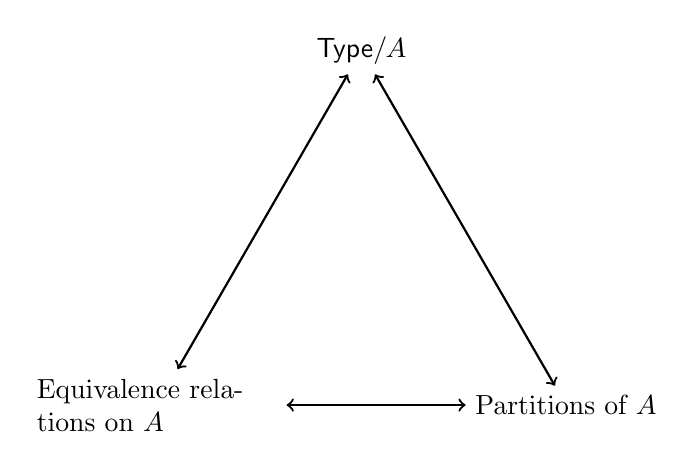
\begin{tikzpicture}
        \node[text width=1.2in] (E) at (-150:3) {Equivalence relations on $A$};
        \node (P) at (-30:3) {Partitions of $A$};
        \node (F) at (90:3) {$\mathsf{Type}/A$};
        \draw[thick,<->] (E) -- (P);
        \draw[thick,<->] (E) -- (F);
        \draw[thick,<->] (F) -- (P);
    \end{tikzpicture}
\end{center}
\end{theorem}